\documentclass[11pt,a4paper]{article}

\usepackage[T1]{fontenc}
\usepackage{lmodern}
\usepackage{microtype}
\usepackage[a4paper,margin=2.5cm]{geometry}
\usepackage{setspace}
\usepackage{graphicx}
\usepackage{xcolor}
\usepackage{booktabs}
\usepackage{tabularx}
\usepackage{longtable}
\usepackage{array}
\usepackage{enumitem}
\usepackage{amsmath,amssymb}
\usepackage{tikz}
\usetikzlibrary{arrows.meta,positioning,fit,shapes.geometric,calc}
\usepackage{caption}
\usepackage{float}
\usepackage[round,authoryear]{natbib}
\usepackage{xurl}
\usepackage{hyperref}

\definecolor{iscteblue}{HTML}{123A63}
\definecolor{lightblue}{HTML}{EAF1F7}
\definecolor{lightgray}{HTML}{F3F4F6}
\hypersetup{
  colorlinks=true,
  linkcolor=iscteblue,
  citecolor=iscteblue,
  urlcolor=iscteblue,
  pdftitle={Network Vulnerability Assessment in a Digital-City Bazaar Pilot},
  pdfauthor={Group project team; member identifiers omitted}
}
\setstretch{1.12}
\setlength{\parskip}{0.45em}
\setlength{\parindent}{0pt}
\setlist[itemize]{leftmargin=1.5em,itemsep=0.2em,topsep=0.3em}
\setlist[enumerate]{leftmargin=1.8em,itemsep=0.25em,topsep=0.3em}
\renewcommand{\arraystretch}{1.2}
\newcolumntype{Y}{>{\raggedright\arraybackslash}X}
\newcolumntype{L}[1]{>{\raggedright\arraybackslash}p{#1}}
\newcommand{\reporttitle}{Network Vulnerability Assessment and Penetration Testing in a Digital-City Bazaar Pilot}
\newcommand{\risk}{\textit{risk}}

\begin{document}

\hypersetup{pageanchor=false}
\begin{titlepage}
\centering
\vspace*{1.3cm}
{\Large\textsc{ISCTE -- Instituto Universit\'ario de Lisboa}\par}
\vspace{0.6cm}
{\large Master in Computer Engineering (B104)\par}
{\large Security in Networks and Information Systems\par}
\vspace{2.1cm}
{\color{iscteblue}\rule{\textwidth}{1.2pt}\par}
\vspace{0.55cm}
{\LARGE\bfseries \reporttitle\par}
\vspace{0.45cm}
{\Large A Kali Linux and Metasploitable 2 Assessment Plan\par}
\vspace{0.55cm}
{\color{iscteblue}\rule{\textwidth}{1.2pt}\par}
\vspace{1.7cm}
{\large\textbf{Group members}\par}
\vspace{0.35cm}
\begin{tabular}{c}
Identities omitted in this repository copy
\end{tabular}
\vfill
\vspace{0.4cm}
{\large 12 November 2026\par}
\end{titlepage}

\hypersetup{pageanchor=true}
\pagenumbering{roman}
\section*{Abstract}
Digital-city services depend on interconnected systems whose security cannot be evaluated by technology lists alone. This report develops a bounded, reproducible plan for assessing a small pilot network associated with the Bazaar district of Lucid Jungles, a conceptual digital city. The pilot is represented by an intentionally vulnerable Metasploitable 2 virtual machine, assessed from Kali Linux inside an isolated VirtualBox host-only network. It is not a functioning city service, payment platform, or production system. The report reviews established security-testing guidance and empirical work on vulnerability scanners, then combines service discovery, cautious vulnerability validation, evidence recording, and contextual risk prioritisation into one method. A simple ordinal risk model is defined as a project heuristic and kept separate from CVSS technical severity. The practical assessment and its results are not reported here because they have not yet been collected. The proposed deliverables are a verified service inventory, evidence-backed findings, a prioritised mitigation plan, and a retest record. The final discussion explains how results from this deliberately small pilot could inform, but cannot prove the security of, a future segmented Bazaar environment.

\textbf{Keywords:} vulnerability assessment; penetration testing; Metasploitable 2; digital city; risk prioritisation

\section*{Glossary and Acronyms}
\begin{tabularx}{\textwidth}{>{\bfseries\raggedright\arraybackslash}p{3cm}Y}
Asset & A system, service, information set, or capability that has value and requires protection.\\
Attack surface & The set of reachable interfaces and services through which a threat could act.\\
CVSS & Common Vulnerability Scoring System, a standard for communicating technical vulnerability severity.\\
CVE & Common Vulnerabilities and Exposures identifier for a publicly disclosed vulnerability.\\
CIA & Confidentiality, integrity, and availability security objectives.\\
Finding & A potential weakness supported by evidence and reviewed for accuracy and scope.\\
Host-only network & A virtual network connecting selected virtual machines to one another and the host, without bridging them onto an external production network.\\
Metasploitable 2 & An intentionally vulnerable Ubuntu virtual machine maintained by Rapid7 for security testing and education.\\
NIST & United States National Institute of Standards and Technology.\\
ROE & Rules of engagement defining approved scope, methods, timing, contacts, and stop conditions for a security test.\\
Synthetic data & Artificial records created for testing that do not identify real people or represent real transactions.\\
\end{tabularx}

\clearpage
\tableofcontents
\clearpage
\pagenumbering{arabic}

\section{Introduction}
\subsection{Context and problem}
Lucid Jungles is treated in this project as a conceptual digital city with connected civic and commercial services, following the group's scenario notes \citep{lucidjungles2026}. Its Bazaar is the setting for the security discussion: a future digital service environment might support merchant listings, storefront information, and related customer interactions. The project does not assume that Lucid Jungles is a deployed system. It also does not test a real marketplace, payment processor, citizen portal, or municipal network.

The approved group project proposes network vulnerability assessment and penetration testing with Kali Linux and Metasploitable 2 \citep{groupproposal2026}. This report gives that approved work a bounded city context. The virtual machine represents a small legacy-service pilot associated with the Bazaar, not the Bazaar itself. It is a controlled stand-in through which the group can practise identifying exposed services, checking evidence, and translating technical observations into defensive priorities. Rapid7 describes Metasploitable 2 as an intentionally vulnerable Ubuntu virtual machine designed for testing security tools and demonstrating common vulnerabilities, and warns against exposing it to hostile networks \citep{rapid7_metasploitable}.

The underlying problem is not simply whether a scanner reports a vulnerability. A useful assessment must establish what is in scope, determine which services are actually reachable, distinguish a detection from a verified weakness, assess the consequences in context, and give the system owner a practical route to reduce risk. NIST's testing guide similarly treats planning, technical testing, analysis, and mitigation as connected parts of an assessment \citep{scarfone2008}. Scanner research also shows why tool output should be interpreted rather than accepted as a complete account of security \citep{alsaleh2017,alazmi2022}.

\subsection{Research questions and objectives}
The report is guided by two questions:
\begin{enumerate}
  \item Which repeatable assessment activities are appropriate for discovering and validating weaknesses in the isolated Metasploitable 2 pilot?
  \item How can evidence from that limited pilot be converted into prioritised, context-aware recommendations for a possible future Bazaar service environment?
\end{enumerate}

To answer these questions, the report has four objectives:
\begin{itemize}
  \item define the city scenario, lab boundary, assets, and exclusions without implying that a real city service was tested;
  \item compare established testing guidance and selected empirical studies of vulnerability scanners;
  \item specify a controlled assessment workflow and a transparent risk-prioritisation heuristic; and
  \item identify what the pilot can inform, what it cannot establish, and how subsequent work could test the proposed mitigations.
\end{itemize}

\subsection{Contribution and structure}
The contribution is a traceable assessment design for a single deliberately vulnerable host in an isolated lab. It connects service-level evidence to a plausible Bazaar risk story while keeping observed lab facts separate from city-level assumptions. Section 2 establishes the scenario and threat context. Section 3 compares related work. Sections 4 and 5 define the assessment method and risk model. Sections 6 and 7 discuss its limits, conclusions, and future work.

\section{Scenario and Theoretical Foundations}
\subsection{Lucid Jungles and the Bazaar pilot}
The city context gives the technical exercise a reason to matter. In a future Bazaar environment, the availability and integrity of merchant listings could affect trust and continuity, while exposure of account or contact information could affect privacy. These are scenario-level concerns, not findings about a real service. The pilot is deliberately narrower: one Metasploitable 2 host, one Kali assessment machine, and a host-only virtual network.

The pilot can represent a legacy civic-service host that supports a small part of a hypothetical Bazaar service. It cannot represent a complete city architecture. In particular, the VM does not provide a production merchant platform, payment processing, or a faithful model of application, database, identity, and edge components. Any later design that includes synthetic merchant or customer records must label them as synthetic and must not introduce real personal or payment data.

\subsection{Assets, trust boundaries, and security objectives}
The primary technical asset in the practical phase will be the Metasploitable 2 virtual machine and the services found to be listening on it. The Kali VM is an assessment system and should not be treated as part of the target asset. Assessment outputs, including scan records and screenshots, are project artefacts that must be stored with care and reviewed before sharing.

For the city interpretation, the hypothetical assets are service availability, integrity of merchant-facing content, and confidentiality of any account or contact information. The CIA objectives provide a concise way to express potential consequences. A single host can support discussion of how one compromised service might affect those objectives, but it does not demonstrate a real multi-service attack path or a city-wide impact.

The host-only network is the main trust boundary. The assessment must remain inside it, with no route to public, university, or operational networks. The target's exact listening services and versions must be established during the practical phase. Rapid7's guide gives an example inventory of services on its image, including file transfer, remote login, web, file sharing, and database services, but that example is not evidence about the group's own VM \citep{rapid7_metasploitable}.

\subsection{Threat model}
The report uses a limited threat model rather than claiming to model every threat to a digital city:
\begin{itemize}
  \item \textbf{Threat actors:} an unauthorised remote user, a malicious or compromised account, or an accidental operator error. These are plausible categories for the scenario, not actors observed in the lab.
  \item \textbf{Threat events:} exploitation of an exposed service, misuse of weak access controls, unauthorised alteration or disclosure of data, or interruption of service.
  \item \textbf{Vulnerable conditions:} outdated software, unnecessary listening services, weak configuration, insecure authentication, or insufficient monitoring. Whether any condition exists on the target remains to be tested.
  \item \textbf{Consequences:} service disruption, loss of integrity, exposure of synthetic test records, or increased effort to restore and verify the service.
\end{itemize}
This framing follows the risk-assessment principle that likelihood and impact depend on threat, vulnerability, and the environment in which a system operates \citep{jointtaskforce2012}.

\section{Related Work and State of the Art}
\subsection{Testing guidance and risk standards}
NIST SP 800-115 provides a practical foundation for planning technical security tests, conducting examinations, analysing findings, and developing mitigation strategies. It also emphasises that different techniques have different benefits and limitations, so a test plan should match the objective and scope \citep{scarfone2008}. This is directly relevant to the proposed pilot: a port scan, a vulnerability scan, and a controlled validation activity produce different kinds of evidence and should not be treated as interchangeable.

NIST SP 800-30 Rev. 1 places assessment within a broader risk-management process and frames results as decision support for selecting responses to risk \citep{jointtaskforce2012}. NIST SP 800-39 further connects information-system risk to organisational and mission-level decisions \citep{jointtaskforce2011}. These sources support the report's separation between technical severity and the hypothetical service consequences in Lucid Jungles. NIST SP 800-122 and the General Data Protection Regulation also inform the decision to keep the pilot free of genuine personal data \citep{mccallister2010,eu2016gdpr}.

These publications are guidance rather than comparative scanner experiments. Their strength is process: they provide vocabulary and decision structure. They do not establish which tool will detect which weakness on this particular virtual machine, nor do they supply results for the proposed Bazaar scenario.

\subsection{Empirical studies of vulnerability scanners}
Early work examined the capabilities and limitations of black-box web application scanners. \citet{bau2010} analysed the state of automated black-box web testing, while \citet{doupe2010} evaluated black-box scanners against web applications. These studies are relevant because they frame automated scanning as a technique whose coverage depends on the application and test conditions, rather than a substitute for scoping and interpretation.

\citet{alsaleh2017} compared open-source web vulnerability scanners and reported meaningful differences between tools' outputs. \citet{alazmi2022} reviewed 90 papers and identified 30 web vulnerability scanners; their review found that only a subset of the surveyed studies offered quantitative assessment, and that reported evaluation approaches and coverage varied. The review also notes a recurring focus on common web vulnerability classes such as SQL injection and cross-site scripting. These findings caution against inferring comprehensive security from a single scanner or from a narrow web-only test.

\citet{abdulghaffar2023} studied a combined approach using Arachni and OWASP ZAP and reported improved recall and F-measure in their evaluated setting. This supports considering complementary tools where the target actually exposes a web application. However, the result belongs to that study's test applications and configuration; it cannot be transferred as a performance claim about Metasploitable 2 or the group's eventual scan.

\subsection{Comparison and research gap}
Table \ref{tab:related-work} compares the selected sources by purpose, method, and relevance to this project. The comparison shows two complementary strands. Standards define how to plan, conduct, and interpret an assessment; empirical studies examine scanner behaviour in bounded test settings. Neither strand, by itself, supplies an evidence-backed risk account for a hypothetical city service.

\begin{table}[H]
\centering
\caption{Comparison of selected guidance and related studies}
\label{tab:related-work}
\small
\begin{tabularx}{\textwidth}{L{2.7cm}L{2.7cm}YY}
\toprule
\textbf{Source} & \textbf{Approach} & \textbf{Main contribution} & \textbf{Limit for this project}\\
\midrule
NIST SP 800-115 \citep{scarfone2008} & Technical testing guidance & Connects assessment planning, test techniques, analysis, and mitigation. & Guidance is not a benchmark and reports no results for this lab.\\
\citet{bau2010} & Analysis of black-box web testing & Provides an early research view of automated web scanner capability. & Web-focused; does not model network-wide service risk or the Bazaar context.\\
\citet{doupe2010} & Empirical black-box scanner evaluation & Evaluates scanner behaviour against web applications. & Results depend on the tested applications, scanner versions, and test conditions.\\
\citet{alsaleh2017} & Comparative assessment of open-source scanners & Demonstrates that scanner outputs should be compared and interpreted. & Limited to the evaluated web scanners and benchmark setup.\\
\citet{alazmi2022} & Systematic literature review & Synthesises scanner studies, tools, and evaluation practices across 90 papers. & The reviewed literature is web-centric and uses heterogeneous evaluation methods.\\
\citet{abdulghaffar2023} & Multi-scanner web testing & Reports gains from combining two scanners in its evaluated setting. & Does not establish that the same gain applies to this target or lab.\\
\citet{rapid7_metasploitable} & Deliberately vulnerable training image and vendor guide & Provides a controlled practice target and example service inventory. & An educational VM is not representative evidence about a production city.\\
\bottomrule
\end{tabularx}
\end{table}

The gap addressed here is therefore practical and contextual, not a claim that the project invents a new scanning technique. The report combines network-service discovery, evidence review, risk prioritisation, and mitigation planning for a deliberately bounded legacy-host pilot. It makes the translation to a possible city environment explicit while limiting conclusions to what the lab can support.

\subsection{Review method and limits}
The literature review is focused and structured, not an exhaustive systematic review. The course's systematic-review protocol informed the use of a defined question, explicit source-selection criteria, and a comparison matrix. Targeted searches and source verification used course materials, Crossref, OpenAlex, and publisher or standards-body pages through 12 November 2026. Search concepts covered black-box web vulnerability scanning, network security testing, penetration testing, vulnerability assessment, and risk assessment.

Included sources were selected for one or more of the following reasons: they are authoritative testing or risk guidance; they report peer-reviewed empirical work on scanners; or they document the intended training target. Sources were excluded from the comparison if their relevance could not be checked from a reliable bibliographic record or accessible abstract. The review does not report database hit counts or screening totals and therefore does not claim systematic-review completeness. The main evidence limitations are the small number of selected empirical studies and their emphasis on web applications rather than mixed network services.

\section{Proposed Assessment Method}
\subsection{Study design and scope}
The practical project is designed as a bounded, controlled technical assessment of one intentionally vulnerable virtual host. The method is based on the testing life cycle in NIST SP 800-115, adapted to the approved VirtualBox host-only arrangement \citep{scarfone2008}. This theoretical report defines the method; it does not report scans, exploit validation, or findings as completed work.

\textbf{In scope:} the assigned Metasploitable 2 VM, its reachable services on the isolated host-only segment, and controlled validation of candidate findings. A limited proof-of-concept exploit may be used only when it is explicitly authorised in the rules of engagement, confined to the target, and recoverable from a snapshot.

\textbf{Out of scope:} public or university networks, any live Lucid Jungles or municipal infrastructure, real payment processing, real merchant or citizen data, denial-of-service testing, persistence, and actions that alter systems outside the target VM. If the agreed scope or network isolation cannot be confirmed, testing must stop.

\subsection{Pilot architecture}
Figure \ref{fig:architecture} shows the intended lab boundary and the relationship between the lab and the city scenario. The dashed city box marks a conceptual service context, not a network connection. Kali is the assessor, Metasploitable 2 is the only target, and the VirtualBox host-only segment isolates the exercise. Other network adapters should be disabled for the target during testing unless the instructor explicitly approves a different configuration. Rapid7 specifically warns that the intentionally vulnerable image should not be exposed to a hostile network \citep{rapid7_metasploitable}.

\begin{figure}[H]
\centering
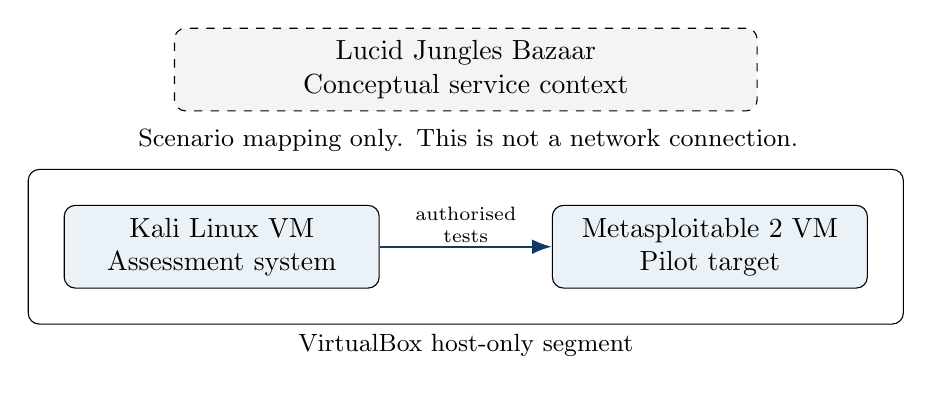
\begin{tikzpicture}[
  box/.style={draw,rounded corners,align=center,minimum width=4.0cm,minimum height=1.05cm,fill=lightblue},
  context/.style={draw,dashed,rounded corners,align=center,minimum width=7.4cm,minimum height=1.05cm,fill=lightgray},
  link/.style={-{Latex[length=2.5mm]},thick,draw=iscteblue}
]
\node[context] (city) at (0,2.25) {Lucid Jungles Bazaar\\Conceptual service context};
\node[align=center,font=\small,text width=10cm] at (0,1.35) {Scenario mapping only. This is not a network connection.};
\node[box] (kali) at (-3.1,0) {Kali Linux VM\\Assessment system};
\node[box] (target) at (3.1,0) {Metasploitable 2 VM\\Pilot target};
\node[draw,rounded corners,fit=(kali)(target),inner sep=0.45cm] (boundary) {};
\draw[link] (kali.east) -- node[above,align=center,font=\scriptsize,fill=white,inner sep=1pt]{authorised\\tests} (target.west);
\node[align=center,font=\small] at (0,-1.25) {VirtualBox host-only segment};
\end{tikzpicture}
\caption{Conceptual city context and isolated assessment boundary}
\label{fig:architecture}
\end{figure}

\subsection{Assessment phases}
The planned phases and their outputs are summarised in Table \ref{tab:phases}. Tool choice should remain proportionate to the target and the approved rules of engagement. A discovery result is not itself a vulnerability finding; a scanner alert is a candidate until it has been checked against service evidence and the target's actual configuration.

\begin{table}[H]
\centering
\caption{Planned assessment phases and evidence}
\label{tab:phases}
\small
\begin{tabularx}{\textwidth}{L{2.4cm}YY}
\toprule
\textbf{Phase} & \textbf{Planned activity} & \textbf{Output}\\
\midrule
1. Authorise and prepare & Confirm written scope, target identity, host-only network, snapshot or recovery point, test window, contacts, and stop conditions. & Approved rules of engagement and a documented baseline.\\
2. Discover & Identify the target and enumerate reachable ports and service banners with a scoped network scanner. & Timestamped service inventory and scan settings.\\
3. Analyse & Check observed service and version evidence against vendor information and vulnerability references. If an HTTP application is present, use a web-testing method suited to the approved scope. & Candidate findings with source, confidence, and evidence references.\\
4. Validate & Manually review candidates. If explicitly authorised, perform the minimum controlled proof-of-concept needed to confirm impact on the target, then restore the agreed baseline. Do not assume scanner output is correct. & Confirmed, rejected, or unresolved findings with rationale.\\
5. Prioritise and recommend & Assess likelihood and impact in the pilot context, record CVSS information when applicable, and propose practical mitigations. & Prioritised risk register and mitigation plan.\\
6. Report and retest & Preserve minimal evidence, document limitations, apply only approved changes, and repeat relevant checks if the practical scope permits. & Final report, retest status, and reproducibility notes.\\
\bottomrule
\end{tabularx}
\end{table}

The approved proposal identifies Nmap, Metasploit Framework, and CVE/CVSS references as intended tools and sources \citep{groupproposal2026}. In this plan, Nmap supports service discovery and Metasploit Framework is reserved for a controlled proof-of-concept against the assigned target when the rules of engagement permit it. An instructor-approved vulnerability or web-application scanner may be added when the discovered services justify its use. Tool names, versions, settings, and scan dates must be recorded in the practical report. No particular service, vulnerability, or scanner result is assumed in advance.

\subsection{Evidence and reproducibility}
Each reported finding should have a unique identifier and, at minimum, the following fields:
\begin{itemize}
  \item affected host and observed service;
  \item evidence source, timestamp, and collection method;
  \item weakness description and supporting CVE or CWE reference, where applicable;
  \item confidence and validation status;
  \item technical severity information, including the CVSS vector when one is assigned;
  \item scenario-specific likelihood, impact, and risk rating;
  \item recommended mitigation, owner, and retest status.
\end{itemize}
The group should preserve raw evidence needed to reproduce a result, but avoid placing passwords, genuine personal information, or unnecessary sensitive output in a shared repository. Screenshots should be redacted if they expose credentials or irrelevant host data. A finding should be marked unresolved if evidence is insufficient, rather than presented as confirmed.

\subsection{Ethics, safety, and privacy}
Testing is limited to the virtual machines and addresses authorised by the instructor. The target must remain isolated from hostile and operational networks. Testing should stop if the target is not the expected VM, if isolation fails, or if an action causes unexpected disruption. These safeguards are consistent with the planning emphasis in NIST SP 800-115 \citep{scarfone2008} and with the scope restrictions required for lawful security work. Portuguese Law No. 109/2009 addresses computer-related crime, including unauthorised access; this report therefore treats explicit permission and a narrow scope as prerequisites, not formalities \citep{portugal2009}.

No real citizen, merchant, or payment data is required. If a later exercise uses sample records, they should be synthetic and should not be derived from identifiable people. The technical assessment cannot establish GDPR compliance; privacy obligations depend on the actual processing context and organisational controls \citep{eu2016gdpr,mccallister2010}.

\section{Risk Model and Expected Outputs}
\subsection{Separating technical severity from contextual risk}
CVSS communicates technical vulnerability severity using Base, Threat, Environmental, and Supplemental metric groups. FIRST recommends that consumers add threat and environmental context when appropriate and consider other organisational factors in their vulnerability-management process \citep{first2023}. A CVSS score is therefore useful evidence, but it is not the complete business or city-service risk score.

For this project, the group proposes a simple ordinal heuristic:
\begin{equation}
R = L \times I,\qquad I = \max(I_C,I_I,I_A)
\label{eq:risk}
\end{equation}
where \(L\) is the likelihood rating from 1 to 5, \(I_C\), \(I_I\), and \(I_A\) are the confidentiality, integrity, and availability impact ratings from 1 to 5, and \(I\) is the highest of those impacts. The maximum is used so that a severe consequence in one security objective is not obscured by averaging it with lower impacts. Equation \ref{eq:risk} is a project-specific prioritisation aid, not a NIST-prescribed formula. It simplifies the broader risk reasoning in NIST SP 800-30 Rev. 1 and must be applied with documented evidence and judgement \citep{jointtaskforce2012}.

\begin{table}[H]
\centering
\caption{Project likelihood and impact scales}
\label{tab:scales}
\small
\begin{tabularx}{\textwidth}{L{1.7cm}L{2.4cm}YY}
\toprule
\textbf{Value} & \textbf{Likelihood} & \textbf{Impact} & \textbf{Interpretation}\\
\midrule
1 & Rare & Negligible & No credible path or only trivial operational effect.\\
2 & Unlikely & Minor & A constrained path or a small, recoverable effect.\\
3 & Possible & Moderate & A plausible path or a material but bounded effect.\\
4 & Likely & Major & A readily usable path or serious service or data impact.\\
5 & Almost certain & Severe & A strongly evidenced path or a critical, broad, or prolonged impact.\\
\bottomrule
\end{tabularx}
\end{table}

The risk bands in Table \ref{tab:bands} make the heuristic repeatable. They do not replace a reasoned explanation. A report should state why a likelihood and impact value were selected and identify uncertainty.

\begin{table}[H]
\centering
\caption{Illustrative risk bands for the project heuristic}
\label{tab:bands}
\begin{tabular}{ccc}
\toprule
\textbf{Score} & \textbf{Band} & \textbf{Response guide}\\
\midrule
1--4 & Low & Track and address through routine hardening.\\
5--9 & Moderate & Schedule a control or configuration change.\\
10--16 & High & Prioritise mitigation and confirm ownership.\\
17--25 & Critical & Escalate promptly and consider service restriction until treated.\\
\bottomrule
\end{tabular}
\end{table}

\subsection{Illustrative city-level scenarios}
Table \ref{tab:scenarios} shows how a technical observation could be discussed in the Bazaar context. These are hypothetical scenarios, not findings or assigned ratings. No CVSS score is assigned because no specific vulnerability has been verified.

\begin{table}[H]
\centering
\caption{Hypothetical scenarios for interpreting future findings}
\label{tab:scenarios}
\small
\begin{tabularx}{\textwidth}{L{3.1cm}YY}
\toprule
\textbf{Possible observation} & \textbf{Potential Bazaar consequence} & \textbf{Example mitigation direction}\\
\midrule
Unnecessary remote service & Larger attack surface and a possible route to service disruption or unauthorised access. & Disable unused services; restrict necessary management interfaces to approved sources.\\
Weak or outdated web service & Possible alteration or unavailability of merchant-facing content, depending on evidence and privilege. & Patch or isolate the affected service; harden configuration; apply least-privilege access.\\
Exposed database service & If a real future application used the same design, stored records could face unauthorised disclosure or modification. & Keep data services off public-facing segments; enforce authenticated, encrypted, narrowly scoped connections.\\
Insufficient logging or recovery evidence & Delayed detection and longer restoration after an incident. & Centralise relevant logs, define alert ownership, and test backups and restoration procedures.\\
\bottomrule
\end{tabularx}
\end{table}

\subsection{Expected deliverables}
The practical phase is expected to produce a service inventory, a table of validated and unresolved findings, supporting evidence, a prioritised risk register, and mitigation recommendations. If the approved practical scope includes retesting, it should also include before-and-after evidence. These are expected outputs, not completed results. The group must replace this forward-looking description with actual measured evidence after conducting the lab assessment.

\section{Discussion}
\subsection{Why the method fits the pilot}
The proposed method is proportionate to a single-host training environment. It starts with scope and asset discovery, then uses analysis and controlled validation rather than treating a scanner's alert as a conclusion. This is consistent with the process orientation of NIST SP 800-115 and with empirical work documenting variation in scanner results \citep{scarfone2008,alsaleh2017,alazmi2022}. The separate risk heuristic then allows the group to explain why an observed technical issue might matter to a service owner without confusing that judgement with CVSS.

The city setting adds a clear line of reasoning: a legacy host is used as a pilot; evidence from that host informs a risk register; recommendations are translated into principles that could be tested in a larger Bazaar design. The relationship is analytical, not operational. The isolated virtual machine has no connection to Lucid Jungles and cannot validate the security of a hypothetical city.

\subsection{Limitations}
Several limits constrain interpretation:
\begin{itemize}
  \item \textbf{Single-host scope:} the pilot cannot represent the identities, networks, workloads, suppliers, or dependencies of a full city.
  \item \textbf{Training image:} Metasploitable 2 is intentionally vulnerable and is not a realistic baseline for a maintained production service.
  \item \textbf{Snapshot in time:} observed services and vulnerabilities depend on the exact image, configuration, and test date.
  \item \textbf{Tool limitations:} scanners can miss weaknesses or report false positives; the selected empirical literature is largely web-focused.
  \item \textbf{Risk-model limitations:} an ordinal product helps prioritise but does not estimate monetary loss, safety consequences, or uncertainty statistically.
  \item \textbf{No results yet:} until the practical assessment is performed, the report cannot state which services were present, which vulnerabilities were confirmed, or whether any mitigation worked.
\end{itemize}

\subsection{Implications for a wider digital city}
The pilot can inform questions for a future Lucid Jungles design: which services should be exposed, how administrative access should be constrained, how application and data services should be separated, what evidence is needed for monitoring, and how a service owner should prioritise remediation. It cannot answer these questions for a production city without additional systems, stakeholders, and representative data. Recommendations should therefore be presented as design implications to test, not as controls already deployed or city-wide assurance.

\section{Conclusions and Future Work}
This report has developed a bounded plan for assessing the approved Kali Linux and Metasploitable 2 project in the context of a hypothetical Lucid Jungles Bazaar pilot. The pilot is a single isolated host used to practise a traceable process: define the scope, identify reachable services, verify candidate weaknesses, record evidence, assess contextual risk, and recommend mitigations. The comparison of standards and scanner studies supports a central methodological choice: automated output is useful evidence, but it needs validation and interpretation.

No practical testing results are claimed here. The exact services, candidate vulnerabilities, confirmed findings, and mitigation effectiveness remain to be established in the authorised lab. Likewise, no conclusion about a functioning Bazaar, real payments, or a wider city network follows from the training VM.

Future work should first complete the approved lab assessment and preserve enough evidence to reproduce its findings. A subsequent pilot could model a more realistic Bazaar service with separate application and database components, synthetic merchant records, and explicit network boundaries. The group could then test whether proposed controls, such as service allow-listing, least-privilege identities, segmentation, logging, and recovery procedures, reduce the risks identified in the first assessment. At a larger scale, the same method could be adapted to connections between Bazaar, identity services, transport, utilities, and other city districts. Such work would require a new scope, representative architecture, stakeholder approval, and separate validation; the present report provides a starting point for that work, not evidence that it has already been done.

\clearpage
\bibliographystyle{plainnat}
\bibliography{references}

\par\medskip
\noindent\textbf{Project repository.} The project source and supporting documentation are available at \url{https://github.com/gosi-dev/lucid-jungles-bazaar-security-assessment}. The repository is private; the course instructor must be granted access for review.

\end{document}
